\chapter{Tangent Vectors}

\section{Motivation}

Consider the following pictures 
\begin{figure}[H]
    \centering
    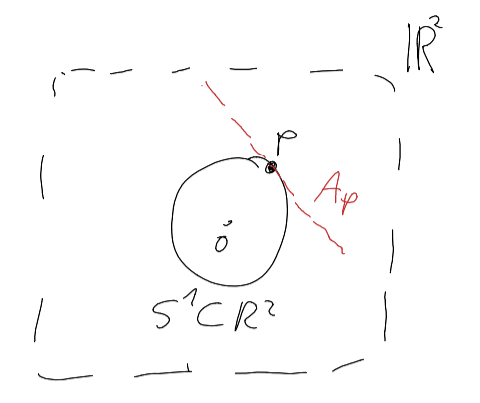
\includegraphics[width=.7\textwidth]{sketch_3_01.png}
    \caption{Sketch 3.01}
\end{figure}
\begin{figure}[H]
    \centering
    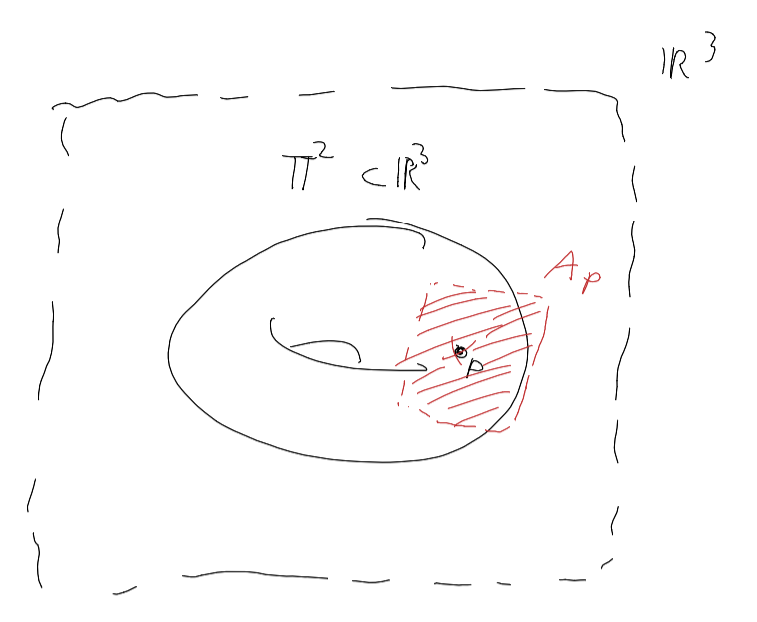
\includegraphics[width=.7\textwidth]{sketch_3_02.png}
    \caption{Sketch 3.02}
\end{figure}
\(A_p\) the affine hyperplane tangent to \(S^1 (\Pi^2)\) at the point \(p\).
Let \(T_p M\coloneqq A_p-p\subset\R^{n+1}\). This is a vector subspace of \(\R^{n+1}\).
It is called the \dhighlight{tangent space of \(M\) at \(p\)}. Consider \[TM=\coprod_{p\in M} T_pM,\]
called the \dhighlight{tangent bundle}. Observe that there is a map 
\marginnote{Think of \(\pi\) as a map of \(p,T_pM\)}
\[\pi:TM\to M\]
by 
\[x\in T_p M\mapsto p\]
the data \(TM\stackrel{\pi}{\to}\) forms a \dhighlight{vector bundle}.

\dhighlight{Problems with this approach:}

\begin{itemize}
    \item not very intrinsic (depends on \(R^{n+1}\)\dots) 
    \item need to prove that manifolds can always embedded into \(R^N\)
\end{itemize}

This is really the picture / intuition we should have, but we will construct it in a different way.

\section{Two (equivalent) theories of tangent vectors} 

\subsection{Definition via equivalence classes of smooth curves}
\marginnote{I could not quite make out what he called this chapter, so I named it according to 
\cite{taylor_equivalent}}

Let \(M\) be a smooth manifold. Fix \(p\in M\). 
\begin{definition*}
    The \dhighlight{tangent space} of \(M\) at \(p\) denoted by \dhighlight{\(T_pM\)} is 
    the set of equivalence classes of smooth curves \(gamma:[-\epsilon,\epsilon]\to M,\gamma(0)=p\)
    with \(\gamma_1\sim\gamma_2\iff\) for any smooth function \(f\) defined near\footnote{in a neighborhood of} \(p\), we have 
    \((f\circ\gamma_1)'(0)=(f\circ \gamma_2)'(0)\). Here the \(\epsilon>0\) is any positive real number, which depends on \(\gamma\).
\end{definition*} 
\begin{figure}[H]
    \centering
    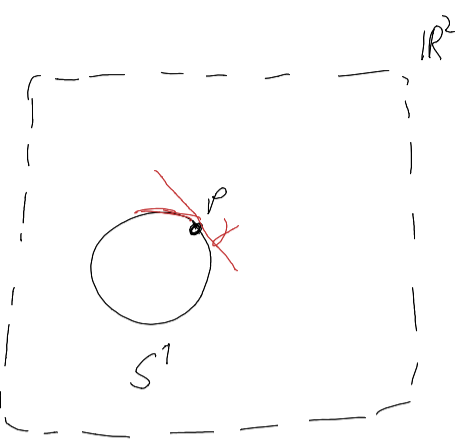
\includegraphics[width=.7\textwidth]{sketch_3_03.png}
    \caption{Sketch 3.03}
\end{figure}

\begin{definition*}
    Given a smooth map \(F:M\to N\), let
    \[dF_p:T_pM\to T_{F(p)}N\]
    be given by \marginnote{This is clearly well defined}
    \[[\gamma]\mapsto [F\circ\gamma].\]
    This map \(dF_p\) is called the \dhighlight{differential of \(F\) at \(p\)}.
\end{definition*}

\begin{remark}
    The map is also called the \dhighlight{tangent map of \(M\) at \(p\)} and the \dhighlight{total derivative}.
    It is also denoted by \[DF_p,TF_p,\nabla F_p,F_p',DF(p),TF(p),\dots\]
\end{remark}

\begin{lemma}[Fundamentality of the differential]\label{lem:3.1}
    Let \(F^1:M_1\to M_2\), \(F^2:M_2\to M_3\) smooth. Then:
    \begin{enumerate}
        \item[(i)]\(dF^2_{F^1(p)}\circ dF_p^1=d(F^2\circ F^1)_p\)
        \item[(ii)] If \(F:M\to M\) is the identity, then \(dF_p=\text{id}\)  
    \end{enumerate}
\end{lemma}

\begin{proof}
    Exercise.
\end{proof}

\markeol{06}
\beginlecture{07}{29.10.2024}

\begin{lemma}\label{lem:3.2}
    Let \(\gamma:[-\epsilon,\epsilon]\to \R^n\) and \(\sigma:(-\delta,\delta)\to \R^n\)
    with \(\gamma(0)=\sigma(0)=p\in\R^n\). Then \(\gamma\sim \sigma\iff \underbrace{\gamma'(0)}_{(\gamma_1'(0),\dots \gamma_n'(0))\in\R^n}=\sigma'(0)\)
\end{lemma}

\begin{proof}
    By abusive notation, we denote by \(x_i\) the map \(\R^n\to\R, (x_1,\dots,x_n)\mapsto x_i\).\marginnote{\(x^i\) might be better (in the sense of the dual space), but \(x_i\) is used in practice}.
    If \(\gamma\sim\sigma\), then \(\gamma^{i'}(0)=(x_i\circ \gamma)'(0)\stackrel{\text{Def.}}{=}(x_i\circ\sigma)'(0)=\sigma^{i'}(0)\implies \gamma'(0)=\sigma'(0)\).

    Conversely, suppose \(\sigma'(0)=\gamma'(0)\). Given any \(f\) smooth defined near \(p\), we have 
    \begin{align*}
        (f\circ \gamma)'(0)&=(\partial_{x_1} f(p),\dots,\partial_{x_n} f(p) )\cdot (\gamma^{1'}(0),\dots,\gamma^{n'}(0))\\
        &=(\partial_{x_1} f(p),\dots,\partial_{x_n} f(p) )\cdot (\sigma^{1'}(0),\dots,\sigma^{n'}(0)) \\
        &=(f\circ \sigma')(0).
    \end{align*}
\end{proof}


\begin{corollary}\label{cor:3.3}
    Let \(V\) be a finite dimensional \(\R\) vector space. Then, for any \(p\in V\), the \dhighlight{canonical} map 
    \begin{align*}
        V&\to T_p V\\
        w&\mapsto [t\mapsto p + tw]
    \end{align*}
    is a bijection.
\end{corollary}

\begin{proof}
If \(V=\R^n\), then this is immediate from lemma \ref{lem:3.2}. In general pick a basis 
to define an isomorphism\footnote{In particular a diffeomorphism} \(F:V\to\R^n\). Then the following diagram commutes:
\begin{figure}[H]
    \centering
    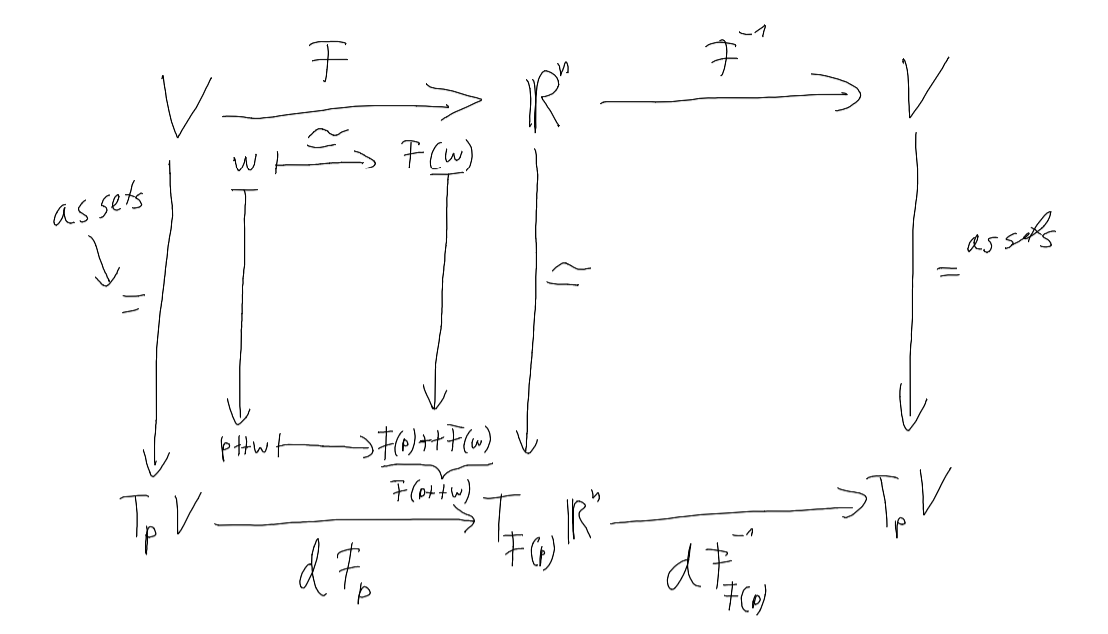
\includegraphics[width=.7\textwidth]{sketch_3_04.png}
    \caption{Sketch 3.04}
\end{figure}    
using lemma \ref{lem:3.1}.
\end{proof}

\subsection{Definition via derivations}

\begin{definition*}
    Let \(M\) be a smooth manifold. A \dhighlight{derivation at \(p\in M\)} is a linear map 
    \[\nu:C^\infty(M)\to\R\]
    satisfying the property 
    \begin{equation}\label{eq:leibniz}\nu(fg)=f(p)\nu(g)+\nu(f)g(p),\end{equation}
    which is also called the \dhighlight{Leibniz rule}.
\end{definition*}
\begin{remark}
    Here \(C^\infty(M)\) is the set of smooth functions from \(f:M\to\R\). It is naturally an \(\R\)-vector space. 
    Similarly we have \(C^0(M)\) the space of continuous functions \(f: M \to \R\) and \(C^k(M)\) the space of \(k\)-times differentiable function \(f:M\to\R\).
\end{remark}
\begin{definition*}
    The set of derivations at \(p\) shall be also called the \dhighlight{tangent space} of \(M\) at \(p\), denoted by \(T_pM\).
\end{definition*}

\begin{lemma}\label{lem:3.4}
    \(T_pM\) is naturally a vector subspace of \(C^\infty(M)^\vee\)\marginnote{\(C^\infty(M)^\vee\) denotes the dual space of \(C^\infty(M)\)}
\end{lemma}
\begin{proof}
    Given derivations \(\nu_1,\nu_2\in T_pM\) we must show that \(a\nu_1+\nu_2\) is still 
    an element of \(T_pM\forall a\in\R\). We compute we compute
    \begin{align*}
        (a\nu_1+\nu_2)(fg)&=a\nu_1(fg)+\nu_2(fg)=a[\nu_1(f)g(p)+f(p)\nu_1(g)]+[\nu_2(f)g(p)+f(p)\nu_2(g)] \\
        &= f(p)[a\nu_1+\nu_2]+[a\nu_1+\nu_2](f)g(p)\qedhere
    \end{align*} 
\end{proof}

\begin{definition*}
    Given a smooth map \(F:M\to N\), we let \(dF_p:T_pM\to T_{F(p)}N\) be the map 
    \[\nu\mapsto dF_p(\nu)\coloneqq C^\infty(N)\ni f\mapsto \nu(f\circ F)\]
\end{definition*}

\begin{lemma}\label{lem:3.5}
    \begin{enumerate}
        \item[(i)] the previous definition gives a derivation 
        \item[(ii)]\(dF^2_{F^1(p)}\circ dF_p^1=d(F^2\circ F^1)_p\)\marginnote{By (ii) and (iii) d is a Functor}
        \item[(iii)] If \(F:M\to M\) is the identity, then \(dF_p=\text{id}\)  
    \end{enumerate}
\end{lemma}

\begin{lemma}\label{lem:3.6}
    Let \(\nu\) be a derivation at \(p\in M\). Then 
    \begin{enumerate}
        \item[(a)] \(f\equiv C\), then \(\nu(f)=0\). That is \(\nu\) annihilates constant functions.
        \item[(b)] if \(f(p)=g(p)=0\), then \(\nu(fg)=0\) 
    \end{enumerate}
\end{lemma}

\begin{proof}
    \dhighlight{(a)}: Since \(\nu\) is linear, it is enough to prove \(\nu(f)=0\) for \(f\equiv 1\). But then 
    \[\nu(f)=\nu(f^2)=f(p)\nu(f)+\nu(f)f(p)=2\nu(f).\]
    \dhighlight{(b)} is obvious by the Leibniz rule (\ref{eq:leibniz}).
\end{proof}

\begin{lemma}\label{lem:3.7} %TODO: check with lee
    Let \(V\) be a finite dimensional vector space over \(\R\). A derivation \(\nu\in T_pV\) is entirely determined by its action 
    on any dual basis \(\{\xi^1,\dots,\xi^n\}\).\marginnote{This should remind us of lemma \ref{lem:3.2}}.     
\end{lemma}

\begin{proof}
    Fix a basis (\(\{e_1,\dots,e_n\}\)) to identify \(V\equiv \R^n\). It is enough to show  
    that \(\nu(f)=0\) if \(\{\partial_{x_1} f(p),\dots,\partial_{x_n} f(p)\}\) all vanish(Indeed, consider \(f\to f-\sum_{k=1}^n \partial_{x_i}f(p)\xi_i\)).\marginnote{with \(\xi_i:\R^n\to\R\) as before}
    By Taylor's formula (Appendix C.15, Lee), we have
    \begin{align*}
        f(x) &= \underbrace{f(p)}_{\text{constant}}+\underbrace{\sum_{i=1}^n\partial_{x_i} f(p)(x_i-p_i)}_{=0}+\sum_{i,j=1}^n \underbrace{(x_i-p_i)}_{\text{constant at }p}\underbrace{(x_j-p_j)\int_0^1 (1-t)\partial_{x_ix_j} f(p+t(x-p)) dt}_{\text{constant at }p}.
    \end{align*}
    Then by lemma \ref{lem:3.6} \(\nu(f)=0\).
\end{proof}

\begin{corollary}\label{cor:3.8} 
    The canonical map \(V\to T_pV\), \(p\in V\)
    defined by 
    \[w\mapsto (C^\infty(V)\ni f\mapsto \frac{d}{dt}\restrict{t=0}f(p+tw))\]
    is an isomorphism of vector spaces.\marginnote{This should remind us of corollary \ref{cor:3.3}}
\end{corollary}

\begin{proof}\marginnote{These are really canonically equal! No choice needed} % TODO: check
    We define \begin{align*}
        T_p V &\to V\\
        \nu&\mapsto \sum_{i=1}^n\nu(\xi^i)e_i,\xi^i:V\to \R
    \end{align*}
    By lemma \ref{lem:3.7} this map is injective and hence \(\dim T_pV \leq \dim V\). So it is enough to show that \(V\mapsto T_pV\) is also injective. 
    Suppose for contradiction that \(V\ni w\neq 0\), that maps to the zero derivation.
    \begin{align*}
        0&=\frac{d}{dt}\restrict{t=0}f(p+tw)\forall f\\
        &\implies 0=\frac{d}{dt}w^\vee(p+tw)=\frac{d}{dt}\restrict{t=0}t=1 \qedhere
    \end{align*}
\end{proof}

\subsection{Both definitions agree}
% fix number and noation
\dhighlight{Temporary notation:} Let \(T_pM^{(1)},dF_p^{(1)}\),\dots, be those objects defined in section 3.2.1 
and  \(T_pM^{(2)},dF_p^{(2)}\),\dots, the analogous objects defined in 3.2.2 

\dhighlight{Key observation:} There is a \dhighlight{canonical} map, for any  \(p\in M\),
\begin{align*}
    K_P:T_pM^{(1)}&\to T_pM^{(2)}\\
    \gamma& \mapsto (C^\infty(M)\ni f\mapsto (f\circ \gamma)'(0)).
\end{align*}
Note that this commutes with \(dF^{(i)}\), i.e. \(dF^{(2)}\circ K_p=K_{F^{(1)}(p)}\circ dF_p^{(1)}\) (exercise).

\begin{proposition}\label{prop:3.9}
    \(K_p\) is a bijection.
\end{proposition}

\begin{proof}
    Choose a chat \((U,\varphi),p\in U\). Then we have a map
    \begin{align*}
        U &\to \varphi(U)\subset R^n\\
    \end{align*}
    \begin{figure}[H]
        \centering
        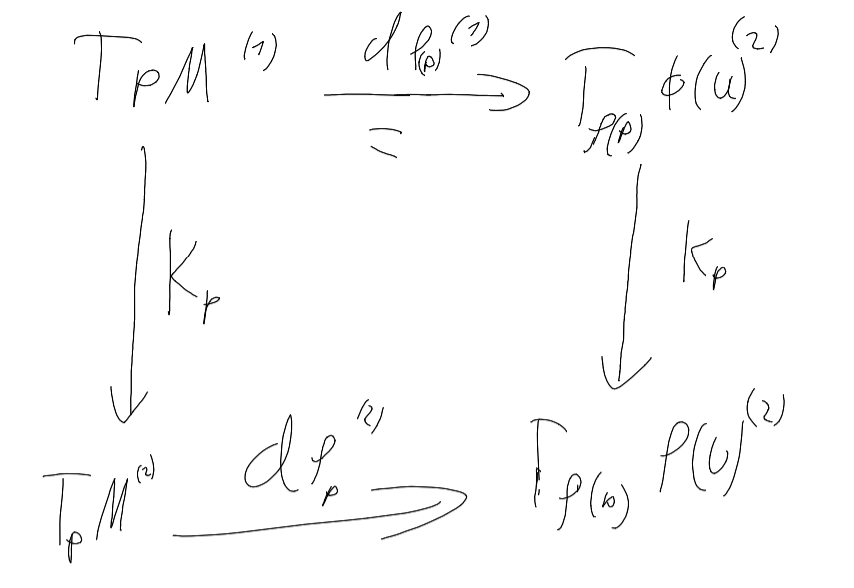
\includegraphics[width=.7\textwidth]{sketch_3_05.png}
        \caption{Sketch 3.05}
    \end{figure}
    Finally, we have 
    \begin{figure}[H]
        \centering
        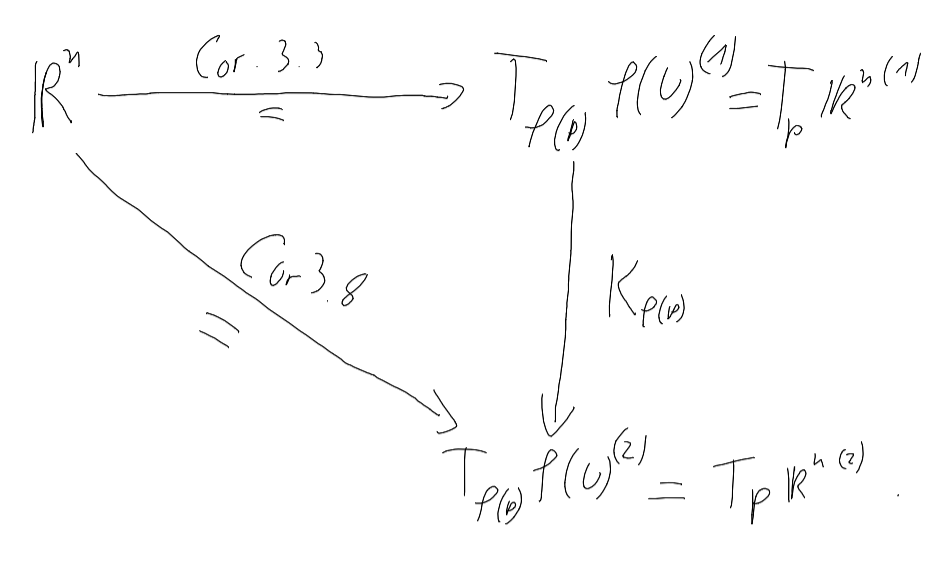
\includegraphics[width=.7\textwidth]{sketch_3_06.png}
        \caption{Sketch 3.06}
    \end{figure}
\end{proof}

\section{Coordinates}

\begin{definition*}
    (1) Given a point \(p\in\R^n\) let \((\partial_{x_i})_p\in T_p\R^n\) be the vector represented by 
    the curve \(t\mapsto p+t\underbrace{(0,\dots,1,\dots,0)}_{e_i}\).

    (2) Given \(p\in M\), we shall abusenotation by writing \((\partial_{x_i})_p\coloneqq d\varphi_{\varphi_p}^{-1}(\partial x_i)_p\) for some chart \(((U,\phi))\) 
\end{definition*}

\begin{remark}
    \begin{enumerate}
        \item Various authors also write \(\partial_{x_i}(p)\)
        \item  \(\{(\partial_{x_1})_p,\dots,(\partial_{x_n})_p\}\) form a basis for \(T_pM\), by construction
        \item \(\{\partial_{x_1},\dots,\partial_{x_n}\}\) very much depend on the chart \((U,\varphi)\)
    \end{enumerate}
\end{remark}

Suppose now that \(F:M\to N\) smooth map. Let \((U,\varphi),(V,\psi)\) be charts, \(F(U)\subset V\). Let 
\(\hat{p}\coloneqq \phi(p)\in\R^m\). Then we have 
\begin{figure}[H]
    \centering
    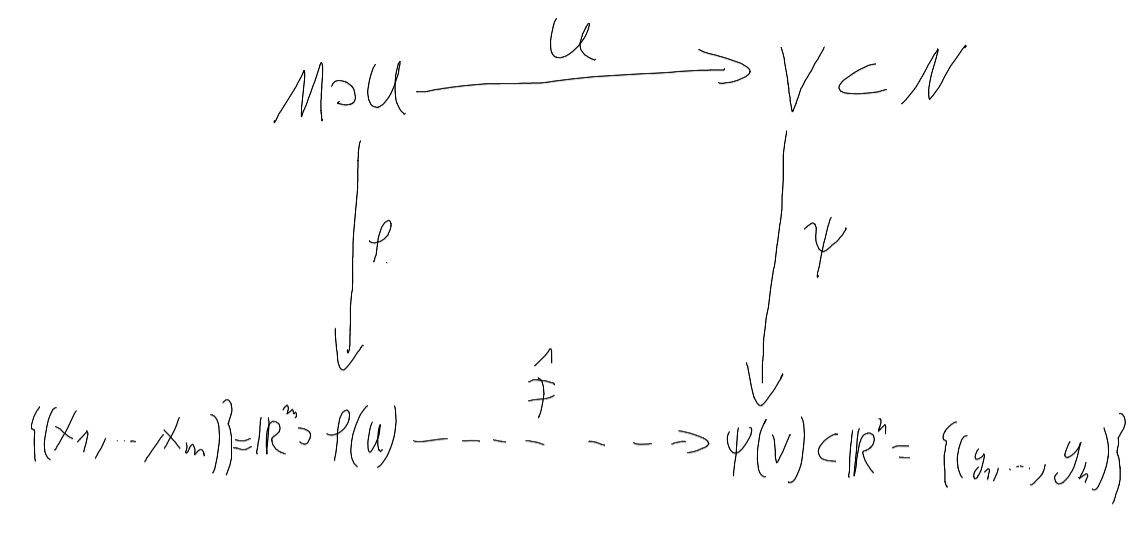
\includegraphics[width=.7\textwidth]{sketch_3_07.png}
    \caption{Sketch 3.07}
\end{figure}
where \(\hat{F}=\psi\circ F\circ \varphi^{-1}\).

Note that \(d\hat{F}_{\hat{p}}:T_{\hat{p}}\R^m\to T_{\hat{F}(\hat{p})}\R^n\) is a linear map. We want to find 
an expression ofr the matrix  \(d\hat{F}_{\hat{p}}\) w.r.t the basis \(\{\partial_{x_1},\dots,\partial_{x_m}\}\) and \(\{\partial_{y_1},\dots,\partial_{y_k}\}\).

Well, by definition
\begin{align*}
    d\hat{F}_{\hat{p}}((\partial_{x_i})_{\hat{p}})&\coloneqq [\hat{F}(\hat{p}+(0,\dots,1,0,\dots 0))]\\
    &=\sum_{j=1}^n \partial_{{x_i}} F^j(\hat{p})(\partial_{y_j})_{\hat{F}(\hat{p})}
\end{align*}

and therefore 
\[d\hat{F}_{\hat{p}}=\begin{pmatrix}
    \partial_{x_1} \hat{F}^1(\hat{p}) & \cdots &\partial_{x_m} \hat{F}^1(\hat{p})\\
    \vdots & & \vdots \\
    \partial_{x_1} \hat{F}^n(\hat{p}) & \cdots &\partial_{x_m} \hat{F}^n(\hat{p})\\
\end{pmatrix}.\]

\markeol{07}
\beginlecture{08}{05.11.2024}

\begin{remark}
    By abuse of notation we often write \(F\equiv \hat{F},p\equiv \hat{p},\partial_{x_i}f\equiv \partial_{x_i}\hat{F}, dF_p\equiv d\hat{F}_{\hat{p}}\)
    \begin{figure}[H]
        \centering
        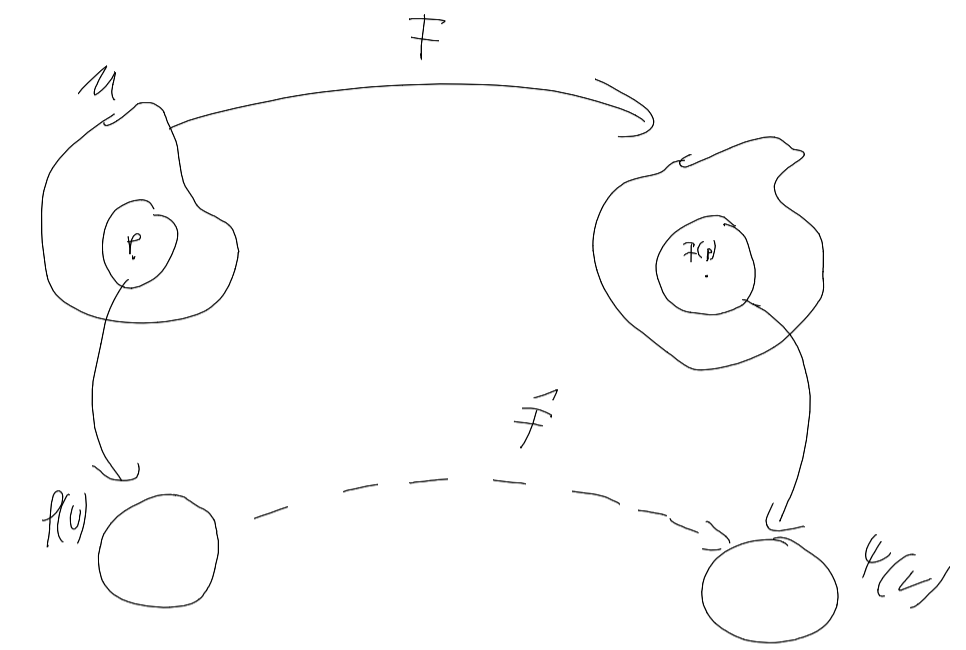
\includegraphics[width=.7\textwidth]{sketch_3_08.png}
        \caption{Sketch 3.08}
    \end{figure}
\end{remark}

\begin{remark}
    \(d\hat{F}_{\cdot}:\underbrace{x}_{\in \phi(U)\subset \R^m}\mapsto d\hat{F}_x\in \text{Mat}(n\times m)\equiv \R^{n\times m}\). This it clearly 
    a smooth map.
\end{remark}

\section{The tangent bundle}

\begin{definition*}
    Given a smooth manifold \(M\), let \(\TM\coloneqq \coprod_{p\in M} T_p M\). We write 
    elements of \(\TM\) as pairs \((p,v)\), where \(v\in T_p M\). Note that we have a map 
    \[\pi:\TM\to M, (p,v)\mapsto p.\]
\end{definition*}

\begin{remark}[Added by Manuel, was an answer to my question]
    For \(p\in M\) the preimage of \(p\) under \(\pi\) is called a \dhighlight{fiber}. 
    He also highlighted, the condition that \(\pi^{-1}(p)\) is a vector space (namely \(T_pM\)),
    which seems to be important in our context, but not generally required for fibers. 
\end{remark}

A priori, TM is just a set. We will exhibit natural smooth manifold structure. 

\dhighlight{Special case:} \(M\subset U\R^n\). Then \begin{align*}
    TU&\coloneqq \coprod_{p\in U} T_p U\equiv U\times \R^n\\
    & (t\mapsto  p+tv)\mapsto(p,v) % fix
\end{align*}\marginnote{Remember that this is a canonical identification!}

\dhighlight{General construction} Given a smooth chart \((U,\phi)\) for a smooth manifold \(M\), we have a map \(d\phi\)
\begin{figure}[H]
    \centering
    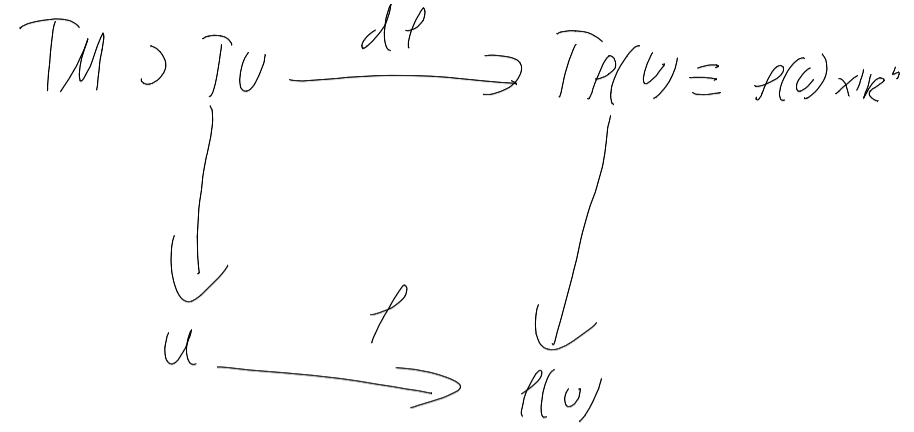
\includegraphics[width=.7\textwidth]{sketch_3_09.png}
    \caption{Sketch 3.09}
\end{figure}
where \[d\phi(p,v)\coloneqq (\phi(p),d\phi_p(v)).\]

Define a subset \(S\subset \TM\) to be open, if, for any chart \(U,\phi\), \(d\phi(S\cap TU)\) open in \(T\phi(U)\equiv \phi(U)\times \R^n\).\marginnote{This is a pullback} % TODO:FIX 
\begin{lemma}\label{lem:2.10}
    This prescription defines a topological space on \(\TM\). Moreover, \(\TM\) is a topological manifold.
\end{lemma}

\begin{proof}
    Omitted. Check transition maps 
    \[d\psi\circ d\phi^{-1}:\phi(U\cap V)\times \R^n\to \psi(U\cap V)\times \R^n\]
    is it an elementary, but tedious proof. 
\end{proof}

\begin{remark}
    Alternatively define the same topology on TM by taking the basis the union over all charts \((U,\phi)\) in your atlas 
    of \(\{d\phi^{-1}(V)\mid V\subset T(\psi(U)) \text{ open}\}\).
\end{remark}

To make TM into a \dhighlight{smooth} manifold, we take as our atlas the set \(\{(TU,d\phi)\}_{(U,\phi)}\),
where \((U,\phi)\) runs over the smooth charts of \(M\). 

\begin{lemma}\label{lem:3.11}
    this is a smooth atlas. 
\end{lemma}

\begin{proof}
    Fix charts \((U,\phi),(V,\psi)\). Then the transition functions take the form 
    \begin{figure}[H]
        \centering
        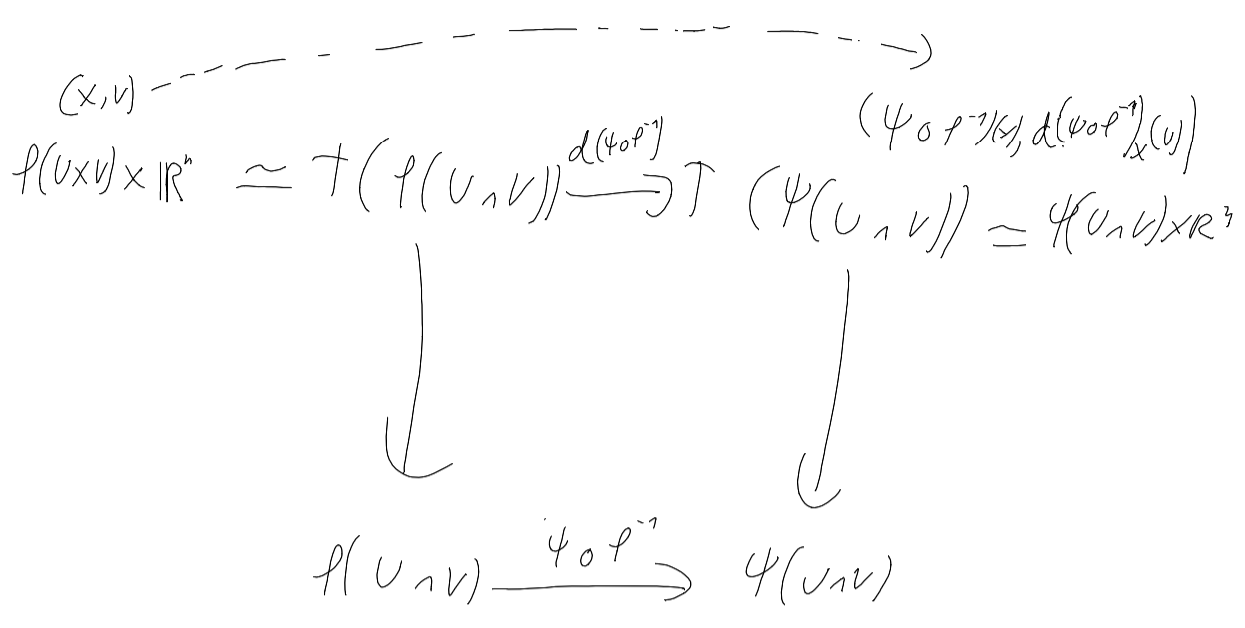
\includegraphics[width=.7\textwidth]{sketch_3_11.png}
        \caption{Sketch 3.11}
    \end{figure}
    Check if both components are smooth:
    \begin{itemize}
        \item The first component \(x\mapsto \psi\circ\phi^{-1}(x)\) is smooth, since \(M\) is a smooth manifold an \((U,\phi),(V,\psi)\) are smooth  \marginnote{Since we can write the second component as a concatination of maps, it is smooth}
        \item For the second component can be fractured as follows: \[(x,v)\mapsto (d(\underbrace{\psi\circ\phi^{-1}_x}_{\in\text{Man}(n\times n)\equiv\R^{2n}},v))\mapsto d(\psi\circ\phi^{-1})_xv\] 
        \dhighlight{Exercise:} the map Mat\((m\times n)\times \text{Mat}(n\times p)\to \text{Mat}(m\times p)\) by \(A,B\mapsto AB\) is smooth. \qedhere
    \end{itemize}
\end{proof}

\begin{remark}
    We will see later %TODO
    that \((\phi:\TM\to M)\) forms a vector bundle. It can be shown that 
    given \(F:M\to N\) the map \(dF:\TM\to\text{TN}, (p,v)\mapsto (F(p),dF_p(v))\) is smooth.\marginnote{This is the exact same computation as in the proof of lemma \ref{lem:3.11}}.

    In fact, we have 
    \begin{figure}[H]
        \centering
        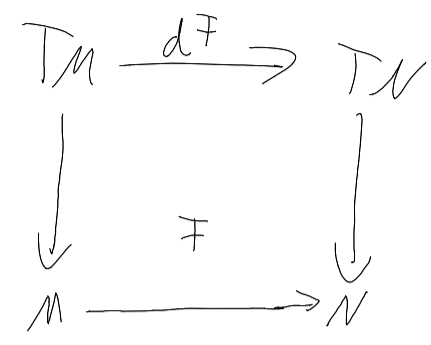
\includegraphics[width=.7\textwidth]{sketch_3_12.png}
        \caption{Sketch 3.12}
    \end{figure}
    commutes. This can be restated as follows: There is a functor \(\maninf\to\text{Smooth vector bundles}\)
    by \[M\mapsto (\pi:\TM\to M)\]
    \[F:M\to N\mapsto dF: \TM \to\text{TN}\]
\end{remark}




